\subsection{Stereo Matching}\label{subsec:stereomatching}

Stereo matching is a technique used to retrieve the depth information out of two rectified images of the same scene by
generating a disparity map.

We will study the approach used by~\citep{stereomatching}.

The disparity at a pixel is the (horizontal) displacement of the pixel in the left image to the pixel representing the
same point in the 3D scene but in the right image.

We denote by $I^r$, $I^g$ and $I^b$ respectively the red, green and blue channels of the image $I$.
Furthermore, the grayscale version of $I$ is denoted $\tilde{I}=0.299\cdot I^r+0.587\cdot I^g+0.0721\cdot I^b$.

The authors give a cost function that models how likely it is that pixel $i=(i_x,i_y)$ in the left image $I_L$ and
pixel $j=(j_x,j_y)$ in the right image $I_R$ are actually projections of the same 3D point onto their respective image
plane.
They define two different costs:
\begin{itemize}
    \item A cost that models the absolute difference in color (if the colors of the two pixels are vastly different, then
    they most likely don't represent the same physical point):
    \[N_{\text{color}}(i,j)=\frac{1}{3}\left(|I_L^r(i)-I_R^r(j)|+|I_L^g(i)-I_R^g(j)|+|I_L^b(i)-I_R^b(j)|\right)\]
    \item A cost that models the difference in $x$-gradient for the two images (if one pixel is close to an edge and
    the other is not, then they most likely don't represent the same physical point):
    \[N_{\text{gradient}}(i,j)=|\nabla_x \tilde{I}_L(i)-\nabla_x \tilde{I}_R(j)|\]
    Where the $x$-gradient is defined as:
    \[\nabla_x\tilde{I}(i)=\frac{\tilde{I}(i_x+1,i_y)-\tilde{I}(i_x-1,i_y)}{2}\]
\end{itemize}
The two costs are then combined with a parameter $0\leq \alpha\leq 1$ that controls the contribution of each of the two
costs to the final cost.
As a sidenote, the two costs are in practice thresholded by respectively $\tau_1$ and $\tau_2$.
\[N(i,j)=(1-\alpha)N_{\text{color}}(i,j)+\alpha N_{\text{gradient}}(i,j)\]

Then, for all possible values of disparity $d\in [d_{\min},d_{\max}]$ we can compute the cost for each pixel $i$ if the
disparity of the pixel was really $d$ (where $i+d$ is notation for $(i_x+d,i_y)$).
\[C(i,d)=N(i,i+d)\]
If we take the line corresponding to the pixel $i$ in the volume, we get a function that gives the cost depending on
the disparity $d$.
The main intuition of stereo matching algorithms is to pick the value of $d$ that minimizes this cost function, and do
so for every pixel in the image.
This approach is essentially the same as what was presented during the lecture.

Slices of the cost volume (for a fixed $d$) are very noisy, which is why the authors of~\citep{stereomatching} implement
a so-called \textit{guided filter}.

\begin{figure}[H]
    \centering
    \captionsetup{justification=centering}
    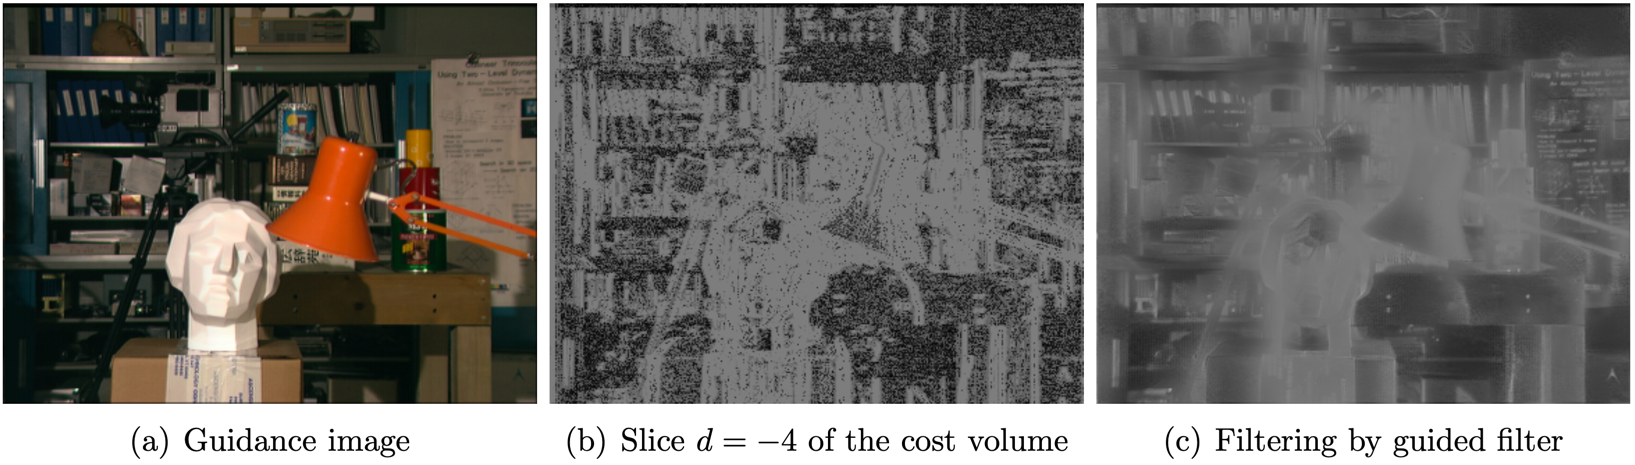
\includegraphics[width=0.9\textwidth]{assets/stereomatching/guidedfiltering}
    \caption{The guided filter (figure from~\citep{stereomatching}).}
    \label{fig:sm_guidedfilter}
\end{figure}

For all pixel $i$ in the image, the filter considers a window around $i$ of a certain radius and uses information from
the original \enquote*{guidance} image (the left input image) to denoise the considered slice of the cost volume.
Hence, for each value of $d$, we can define the \textit{filtered} cost to be $C^{\text{filt}}(i,d)$, the value of the
pixel corresponding to pixel $i$ in the $d$th slice of the filtered cost volume.

In particular, the disparity value that is returned for a pixel $i$ is:
\[d(i)=\argmin_{d'\in [d_{\min},d_{\max}]}\left\{C^{\text{filt}}(i,d')\right\}\]

The authors finally check if the disparity found is constistent: the disparity from the left to the right image is
rejected if the disparity of the corresponding pixel in the right image is different.
That is, the disparity is rejected if the map from the left to the right image disagrees on the disparity with the
map from the right to the left image or if (for $d'(i)$ the disparity of pixel $i$ from right to left):
\[d(i)\neq -d'(i+d(i))\]

\begin{figure}[H]
    \centering
    \captionsetup{justification=centering}
    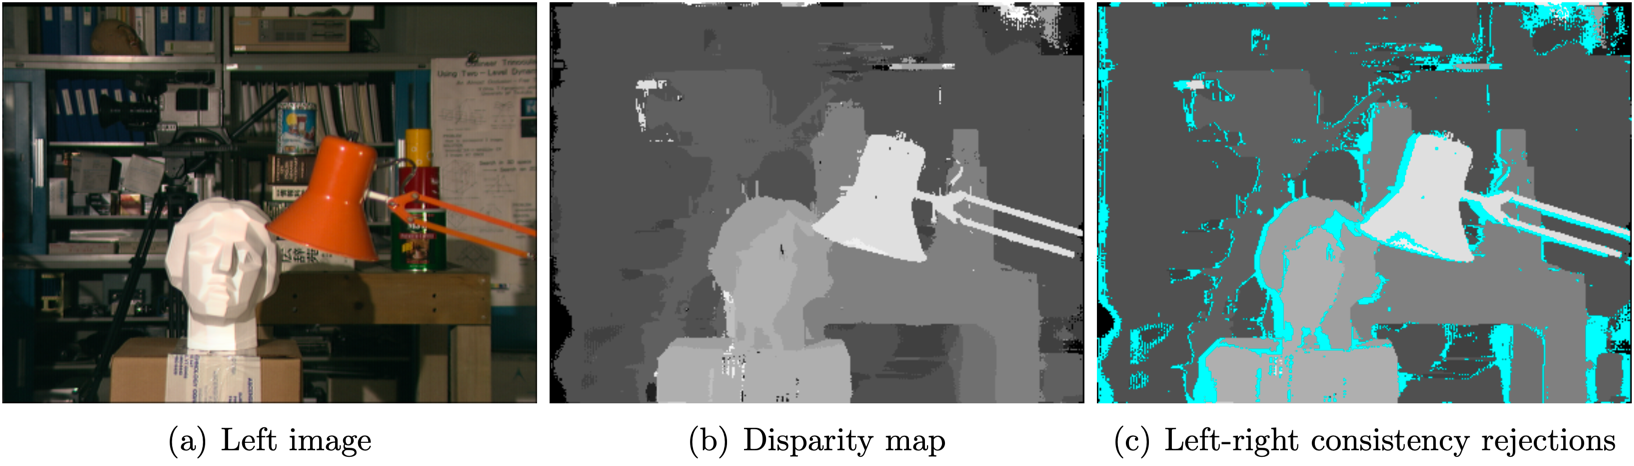
\includegraphics[width=0.9\textwidth]{assets/stereomatching/leftrightconsistency}
    \caption{Left-right consistency rejections (figure from~\citep{stereomatching}).}
    \label{fig:sm_leftrightconsistency}
\end{figure}

In particular, pixels representing occluded points in either image will necessarily be rejected.
It could also happen that a disparity value is rejected on textureless regions, where multiple pixels in the right
image could correspond to the pixel we are looking for in the left image.
To do inpainting, we consider a square window $\omega_i$ or a certain radius around the occluded pixel $i$.
The authors propose the following weight function, that is bigger for disoccluded points $j$ spatially close to $i$ and
for $j$ with a color close to the color of $i$ ($w_s,w_c$ are chosen weights):
\[W_{ij}=e^{-\frac{\left\|i-j\right\|^2}{w_s^2}}\cdot
e^{-\frac{\left\|I_{L,\text{filt}}(i)-I_{L,\text{filt}}(j)\right\|^2_c}{w_c^2}}\]
Then, they define the function $h(d)$ that simply sums all the weights of points $j$ in the window that are at a depth
at most $d$.
\[h(d)=\sum_{j\in\omega_i,d(j)\leq d} W_{ij} \]
Notice that in particular, $h(d)\leq h(d+1)$ for all $d$ (which means that taking the $d$ that maximizes $h$ does not
make any sense).
The value of $d$ that is chosen for occluded $i$ is the one that gives the median of $h$.
This means that if most of the weight is around some depth $d^*$, then a disparity value close to $d^*$ will be chosen
(which makes sense since we have high weights for pixels close in color and in space, we expect the disparity of the
occluded point to be close to the one of these pixels, \textit{QS.5}).

\begin{figure}[ht]
    \centering
    \captionsetup{justification=centering}
    \begin{minipage}{.5\textwidth}
        \centering
    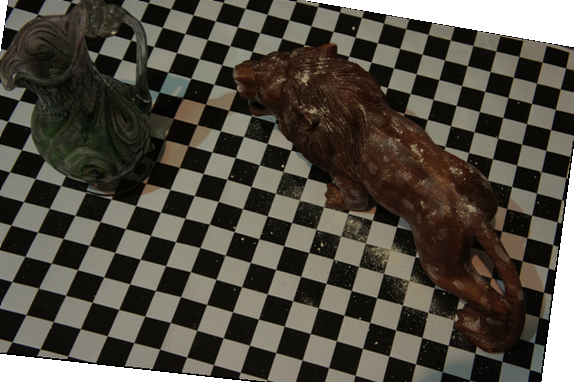
\includegraphics[width=0.7\textwidth]{assets/stereomatching/rect_lion_left}
    \end{minipage}%
    \hfill
    \begin{minipage}{.5\textwidth}
        \centering
    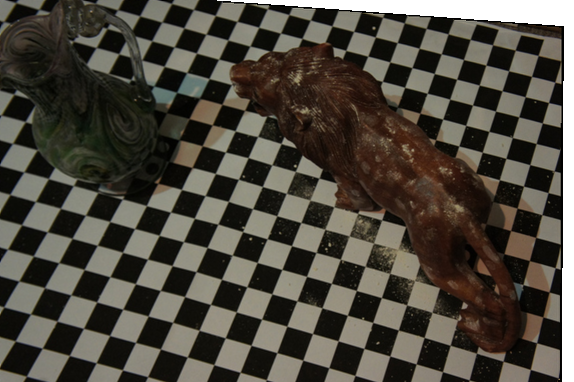
\includegraphics[width=0.7\textwidth]{assets/stereomatching/rect_lion_right}
    \end{minipage}
    \caption{Rectified left and right input images.}
    \label{fig:sm_input}
\end{figure}

We have run the online demo of paper~\citep{stereomatching} on the (rectified) images of figure~\ref{fig:sm_input}.
Figure~\ref{fig:sm_output} shows the output of the algorithm along with the occlusion map and an alternative result
of the algorithm with a simpler inpainting algorithm, where the final disparity value for an occluded pixel $i$ is
the disparity value of the first disoccluded pixel straight to the left or to the right.

\begin{figure}[ht]
    \centering
    \captionsetup{justification=centering}
    \begin{minipage}{.33\textwidth}
        \centering
    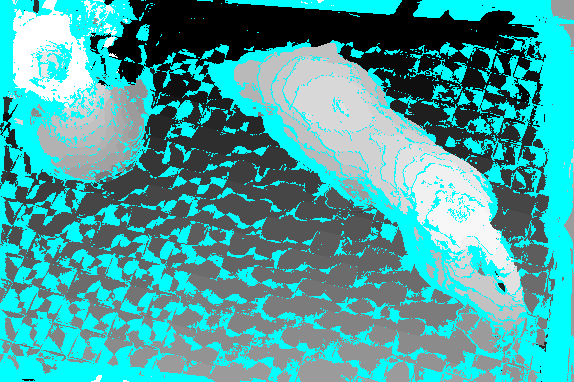
\includegraphics[width=0.95\textwidth]{assets/stereomatching/occlusion_map}
    \end{minipage}%
    \hfill
    \begin{minipage}{.33\textwidth}
        \centering
    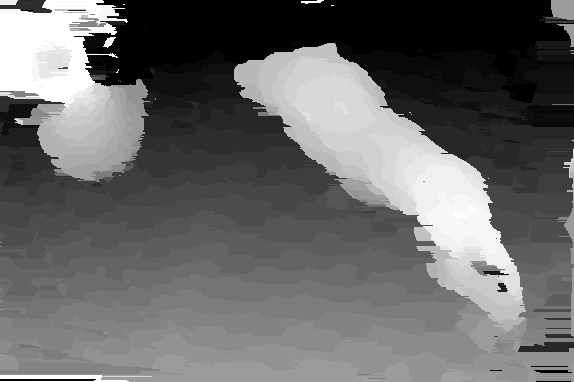
\includegraphics[width=0.95\textwidth]{assets/stereomatching/simple_filling}
    \end{minipage}%
    \hfill
    \begin{minipage}{.33\textwidth}
        \centering
    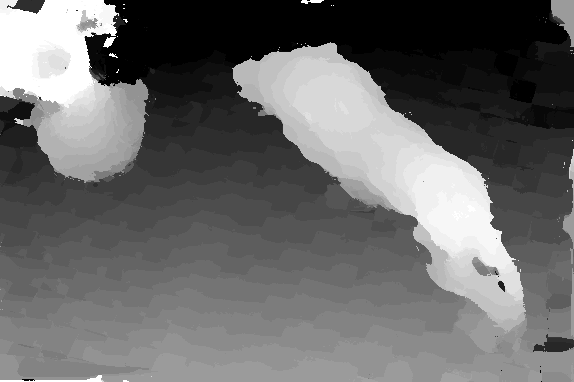
\includegraphics[width=0.95\textwidth]{assets/stereomatching/disparity_map_out}
    \end{minipage}
    \caption{Outputs of the stereo matching of figure~\ref{fig:sm_input}.
    The map with the occluded pixels in blue is on the left, the map after a simple example fill in the center and the
    final map on the right.}
    \label{fig:sm_output}
\end{figure}

We can observe in figure~\ref{fig:sm_output} that a lot of pixels that are not occluded in either images have their
disparity value rejected.
This is because the checkerboard does not have a lot of texture and many parts are monochrome.
In monochrome regions, a large range of disparity values are possible for these pixels and there is no
reason that the disparity values found from left to right and from right to left are the same.

The output map is a disparity map and not a depth map, since the pixels closer to the camera are white (and are thus
of higher value, \textit{QS.2}).
Notice that the disparity map is of poor quality along the (especially right) border of the map.
This is because there are no pixels that represent the same actual point in the right image (\textit{QS.1}).

We can observe that the handle of the vase is not correctly detected by the stereo matching algorithm.
This could be explained by the non-lambertian nature of said handle (and the whole vase in general).
The inner part of the handle is very reflective, which could easily break the algorithm.
The left side of the vase is also badly reconstructed in the disparity map because it is cut off in the
right image: it is on the very border of the image (\textit{QS.3}).

Take a look at section~\ref{subsec:viewsynthesis} and~\ref{subsec:icp} for results with our own figures (\textit{QS.4}).